%%%%%%%% ICML 2018 EXAMPLE LATEX SUBMISSION FILE %%%%%%%%%%%%%%%%%

\documentclass{article}

% Recommended, but optional, packages for figures and better typesetting:
\usepackage{microtype}
\usepackage{graphicx}
\usepackage{subfigure}
\usepackage{booktabs} % for professional tables

% hyperref makes hyperlinks in the resulting PDF.
% If your build breaks (sometimes temporarily if a hyperlink spans a page)
% please comment out the following usepackage line and replace
% \usepackage{icml2018} with \usepackage[nohyperref]{icml2018} above.
\usepackage{hyperref}

% Attempt to make hyperref and algorithmic work together better:
\newcommand{\theHalgorithm}{\arabic{algorithm}}

% Use the following line for the initial blind version submitted for review:
% \usepackage{icml2018}

% If accepted, instead use the following line for the camera-ready submission:
\usepackage[accepted]{icml2018}

% Macros
\newcommand{\todo}{\textbf{\textit{TO~DO: }}}


% The \icmltitle you define below is probably too long as a header.
% Therefore, a short form for the running title is supplied here:
\icmltitlerunning{Reinforcement Learning for Hanabi}

\begin{document}

\twocolumn[
\icmltitle{Reinforcement Learning for Hanabi \\ (Project Milestone)}

\icmlsetsymbol{equal}{*}

\begin{icmlauthorlist}
  \icmlauthor{Vinson Luo}{stanford}
  \icmlauthor{Arthur Tsang}{stanford}
  \icmlauthor{Christopher Yeh}{stanford}
\end{icmlauthorlist}

\icmlaffiliation{stanford}{Department of Computer Science, Stanford, California, USA}

\icmlcorrespondingauthor{Vinson Luo}{vluo@stanford.edu}
\icmlcorrespondingauthor{Arthur Tsang}{atsang@stanford.edu}
\icmlcorrespondingauthor{Christopher Yeh}{chrisyeh@stanford.edu}


% You may provide any keywords that you
% find helpful for describing your paper; these are used to populate
% the "keywords" metadata in the PDF but will not be shown in the document
\icmlkeywords{Deep Reinforcement Learning, Game Playing}

\vskip 0.3in
]

% this must go after the closing bracket ] following \twocolumn[ ...

% This command actually creates the footnote in the first column
% listing the affiliations and the copyright notice.
% The command takes one argument, which is text to display at the start of the footnote.
% The \icmlEqualContribution command is standard text for equal contribution.
% Remove it (just {}) if you do not need this facility.

\printAffiliationsAndNotice{}  % leave blank if no need to mention equal contribution
% \printAffiliationsAndNotice{\icmlEqualContribution} % otherwise use the standard text.

\begin{abstract}
  Hanabi is a collaborative card game where players can only see other players' cards and must rely on limited hints to share information.
  In this project, we approach Hanabi using the reinforcement learning technique of deep Q-networks (DQNs).
  We have implemented a simulator and feature representation of states, with preliminary results in progress.
  In the future, we'd like to add more subtle features to our representations as well as experiment with alternative approaches such as RNNs that can absorb information turn by turn.
\end{abstract}



\section{Introduction}

Hanabi is a cooperative card game where all players can see the other players' hands, but not their own. Instead, one must infer about one's hand through specific hints from others.

In particular, Hanabi is played by 2-5 players using a specialized deck. The goal of the game is to play cards numbered 1 to 5 in sequential order in 5 different suits (as shown in Figure~\ref{fig:cards}), with the score for all players at the end of a game being the number of cards successfully played, for a maximum of 25. It is noted that some luck is involved -- certain initial shuffles of the deck can result in games where a perfect score is unattainable. Each player is dealt a hand of 4-5 cards, but players can only see the hands of other players, not their own. Players take turns taking one of three actions: they can either give a hint to another player (naming all the cards of a given color or number in the other player's hand), play a card from their own hand, or discard a card from their own hand. The players as a whole start with 8 communal hint tokens, which are expended as hints are given and can only be replenished by discarding cards or playing 5’s. Additionally, if a player attempts to play a card which is not actually playable, the play counts as a mistake, and the game ends prematurely after the third mistake.

\begin{figure}
  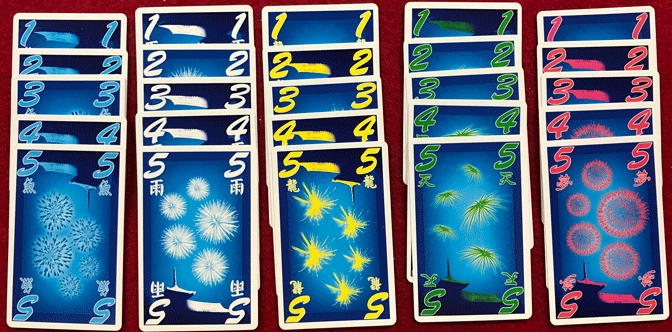
\includegraphics[width=\columnwidth]{cards}
  \label{fig:cards}
  \caption{The Hanabi deck consists of cards numbered 1-5 in 5 different suits, as shown above. The arrangement shown above would give a perfect score of 25.}
\end{figure}

We argue that Hanabi is a particularly interesting arena to develop a cooperative AI agent. First, optimal play requires a theory of mind: since hints are limited, one must understand not only the information conveyed, but why a hint was considered by the other player to be the most informative or useful choice possible at a given point in time. Indeed, this game has been suggested as a measure of social intelligence \cite{osawa15}. Secondly, while many other games like Catan allow a subtle range of natural language communication, in Hanabi, every action, including the range of possible hints, is perfectly well-defined. Lastly, the game is not ``too easy'' in that a brute force approach would not work: not only is there an exponentially large number of possible hands and hints to remember, but even the ordering of hints can contain vital information.


\section{Approach}

Given the success of reinforcement learning in other games \cite{mnih15, silver17}, we approach Hanabi as a reinforcement learning problem, and in particular, at least to start, with a deep Q-network (DQN). Since Hanabi is cooperative, we can optimize a single policy for all players without a separate model for adversarial play. Existing literature has mostly focused on specific information-theoretic analyses of the game. Cox et al., for example, developed the “hat protocol,” a hint protocol that encodes recommended actions or other information beyond the information in the hint itself \cite{cox15}. Baffier et al. have shown that determining whether or not a shuffled Hanabi deck can lead to a perfect score is an NP-complete problem \cite{baffier16}. By using reinforcement learning, we hope to create a model that will generalize well to other variants of the game, or perhaps one which also plays well with humans. We will be able to evaluate the progress of our AI by measuring the average score obtained by a simulator we built.

The game poses many levels of interesting strategy, with multiple possible state space representations. The size and presence of interactions in even a basic state space (which could be comprised of the identity of discarded cards as well as the history of hints) is large enough to warrant the use of deep learning. Later, we will experiment representing states with an RNN-type network which can read the history of actions at every turn. But to get started with something easier to train, we will treat each input state as a feature vector.

Our baseline feature space includes the following features:
\begin{enumerate}
\item Other players' cards and hints:
  \begin{itemize}
  \item For each card, a one-hot vector of colors and numbers (length 10).
  \item For each card, a one-hot vector of if a color or number hint was given (length 2).
  \end{itemize}
\item Own cards and hints:
  \begin{itemize}
  \item For each card, a one-hot vector of which colors and numbers are still possible (length 10).
  \item For each card, a one-hot vector of if a color or number hint was given (length 2).
  \end{itemize}
\item Number of communal hint tokens left, number of mistakes left.
\item Cards which have been successfully played:
  \begin{itemize}
  \item For each suit, a one-hot vector indicating how many cards have been played so far (length 5, using $\mathbf{0}$ if no cards have been played yet).
  \end{itemize}
\end{enumerate}
In addition, we tag each card using a high-level notion very helpful to humans, namely whether a card is playable, indispensable, or dead \cite{cox15}. These are defined as follows:
\begin{description}
\item[Playable] means that a card is valid to be played immediately without counting as a mistake.
\item[Indispensable] means that a card is the last remaining of its suit and number and must eventually be played in order to achieve a perfect score. Even without counting cards, since there is only one 5-card in each suit, one can tell a priori that these are indispensable.
\item[Dead] means that a card of the same type has already been played, so it will never be playable and is perfectly safe to discard.
\end{description}
Of course, a card is not always in one of the three states, and even if it is, it may not be apparent from a given player's point of view, but these notions give a sense of the kind of information that makes a good hint.

We have already implemented and begun to test the above feature space, and while it includes the most intuitively important information, there are still some relevant features that it leaves out. We would like to test a more advanced feature set which includes the features enumerated above, as well as:
\begin{enumerate}
  \setcounter{enumi}{4}
\item Cards remaining in deck:
  \begin{itemize}
  \item A count for each of the 25 types of cards remaining, from the player's point of view.
  \end{itemize}
\item When each hint was given:
  \begin{itemize}
  \item This information proves crucial for more advanced strategies in human play. Due to the constraints of the DQN architecture, it would have a finite length set by a hyperparameter, which represents a horizon beyond which our model no longer remembers when exactly a hint was given.
  \end{itemize}
\end{enumerate}


In addition, we implemented a replay buffer to better decorrelate $(s,a,s')$ triplets. That said, care must be taken to limit the staleness that comes from the fact that the same state implies vastly different information as a policy changes.

Having recently implemented a Hanabi simulator and baseline feature space, as well as a DQN model to train on it, we are in theory ready to present preliminary results. However, our low scores around 1 to 2 indicate that we may need to look harder for bugs or small design flaws.



\bibliography{report}
\bibliographystyle{icml2018}

\end{document}


% This document was modified from the file originally made available by
% Pat Langley and Andrea Danyluk for ICML-2K. This version was created
% by Iain Murray in 2018. It was modified from a version from Dan Roy in
% 2017, which was based on a version from Lise Getoor and Tobias
% Scheffer, which was slightly modified from the 2010 version by
% Thorsten Joachims & Johannes Fuernkranz, slightly modified from the
% 2009 version by Kiri Wagstaff and Sam Roweis's 2008 version, which is
% slightly modified from Prasad Tadepalli's 2007 version which is a
% lightly changed version of the previous year's version by Andrew
% Moore, which was in turn edited from those of Kristian Kersting and
% Codrina Lauth. Alex Smola contributed to the algorithmic style files.

%%% Local Variables:
%%% mode: latex
%%% TeX-master: t
%%% End:
